% !TEX TS-program = lualatex
% !BIB TS-program = biber
%\documentclass[handout]{beamer}
\documentclass{beamer}
\newcommand{\misoclasstinytitleslide}{Partially based on material by:  Rob Fergus, Nikhil Srivastava,\\[-1em] 
Yiannis Koutis, Joshua Batson, Daniel Spielman}
%{Partially based on material by:  Branislav Kveton,  \\[-1em]  Partha Niyogi, Rob Fergus}
\newcommand{\misoclassdate}{}
\input{../common/misomva}
\usepackage{verbatim}
\usepackage{listings}
\usepackage[customcolors]{hf-tikz}
\usepackage{color}
\usepackage{cancel}
%\usepackage[defaultmono]{droidmono}
\newcommand{\nbskip}{\vspace{-\baselineskip}}
%\newcommand{\hbskip}{\vspace{.5\baselineskip}}
\newcommand{\nhbskip}{\vspace{-.5\baselineskip}}

\definecolor{mygreen}{rgb}{0,0.6,0}
\definecolor{mygray}{rgb}{0.5,0.5,0.5}
\definecolor{mymauve}{rgb}{0.58,0,0.82}

\definecolor{Code}{rgb}{0,0,0}
\definecolor{Decorators}{rgb}{0.5,0.5,0.5}
\definecolor{Numbers}{rgb}{0.5,0,0}
\definecolor{MatchingBrackets}{rgb}{0.25,0.5,0.5}
\definecolor{Keywords}{rgb}{0,0,1}
\definecolor{self}{rgb}{0,0,0}
\definecolor{Strings}{rgb}{0,0.63,0}
\definecolor{Comments}{rgb}{0,0.63,1}
\definecolor{Backquotes}{rgb}{0,0,0}
\definecolor{Classname}{rgb}{0,0,0}
\definecolor{FunctionName}{rgb}{0,0,0}
\definecolor{Operators}{rgb}{0,0,0}
\definecolor{Background}{rgb}{0.98,0.98,0.98}

\newcommand{\fdmfamily}{\ttfamily}

\lstset{ %
backgroundcolor=\color{white},   % choose the background color; you must add \usepackage{color} or \usepackage{xcolor}
basicstyle=\fdmfamily\footnotesize,        % the size of the fonts that are used for the code
breakatwhitespace=false,         % sets if automatic breaks should only happen at whitespace
breaklines=true,                 % sets automatic line breaking
captionpos=b,                    % sets the caption-position to bottom
commentstyle=\color{mygreen},    % comment style
deletekeywords={\dots},            % if you want to delete keywords from the given language
escapeinside={\%*}{*)},          % if you want to add LaTeX within your code
extendedchars=true,              % lets you use non-ASCII characters; for 8-bits encodings only, does not work with UTF-8
frame=single,	                   % adds a frame around the code
keepspaces=true,                 % keeps spaces in text, useful for keeping indentation of code (possibly needs columns=flexible)
language=Python,                 % the language of the code
% Comments
commentstyle=\color{Comments}\slshape,
% Strings
stringstyle=\color{Strings},
morecomment=[s][\color{Strings}]{"""}{"""},
morecomment=[s][\color{Strings}]{'''}{'''},
% keywords
morekeywords={import,from,class,def,for,while,if,is,in,elif,else,not,and,or,print,break,continue,return,True,False,None,access,as,,del,except,exec,finally,global,import,lambda,pass,print,raise,try,assert},
keywordstyle={\color{Keywords}\bfseries},
% additional keywords
morekeywords={[2]@invariant},
keywordstyle={[2]\color{Decorators}\slshape},
emph={self},
emphstyle={\color{self}\slshape},
otherkeywords={*,\dots},            % if you want to add more keywords to the set
numbers=left,                    % where to put the line-numbers; possible values are (none, left, right)
numbersep=5pt,                   % how far the line-numbers are from the code
numberstyle=\tiny\color{mygray}, % the style that is used for the line-numbers
rulecolor=\color{black},         % if not set, the frame-color may be changed on line-breaks within not-black text (e.g. comments (green here))
showspaces=false,                % show spaces everywhere adding particular underscores; it overrides 'showstringspaces'
showstringspaces=false,          % underline spaces within strings only
showtabs=false,                  % show tabs within strings adding particular underscores
stepnumber=1,                    % the step between two line-numbers. If it's 1, each line will be numbered
tabsize=2,	                   % sets default tabsize to 2 spaces
title=\lstname                   % show the filename of files included with \lstinputlisting; also try caption instead of title
}


\newcommand{\consindent}[1]{
    \begin{itemize}
        \item[{
\includegraphics[height=0.7\baselineskip]{../img/arrow_list}}] #1
    \end{itemize}
}


%%% part daniele
\usepackage{etex}
\TPshowboxesfalse
\textblockorigin{0mm}{0mm}

\definecolor{rouge1}{RGB}{226,0,38}  % red P
\definecolor{orange1}{RGB}{243,154,38}  % orange P
\definecolor{jaune}{RGB}{254,205,27}  % jaune P
\definecolor{blanc}{RGB}{255,255,255} % blanc P

\definecolor{rouge2}{RGB}{230,68,57}  % red S
\definecolor{orange2}{RGB}{236,117,40}  % orange S
\definecolor{taupe}{RGB}{134,113,127} % taupe S
\definecolor{gris}{RGB}{91,94,111} % gris S
\definecolor{bleu1}{RGB}{38,109,131} % bleu S
\definecolor{bleu2}{RGB}{28,50,114} % bleu S
\definecolor{vert1}{RGB}{133,146,66} % vert S
\definecolor{vert3}{RGB}{20,200,66} % vert S
\definecolor{vert2}{RGB}{157,193,7} % vert S
\definecolor{darkyellow}{RGB}{233,165,0}  % orange S
\definecolor{lightgray}{rgb}{0.9,0.9,0.9}
\definecolor{darkgray}{rgb}{0.6,0.6,0.6}

\setbeamertemplate{navigation symbols}{}
\setbeamertemplate{blocks}[rounded]
\setbeamercolor{block title}{bg=bleu2,fg=white}%bg=background, fg= foreground
\setbeamercolor{block body}{bg=lightgray}%bg=background, fg= foreground

\renewcommand{\sfdefault}{lmss}
\sffamily

%\newcommand{\ycol}[1]{\textcolor{darkyellow}{\textit{#1}}}

\newcommand{\rcolb}[1]{\textcolor{red}{\textit{\textbf{#1}}}}
\newcommand{\gcolb}[1]{\textcolor{vert3}{\textit{\textbf{#1}}}}
\newcommand{\bcolb}[1]{\textcolor{blue}{\textit{\textbf{#1}}}}
\newcommand{\ycolb}[1]{\textcolor{darkyellow}{\textit{\textbf{#1}}}}

\newcommand{\eqrcol}[1]{\textcolor{red}{#1}}
\newcommand{\eqgcol}[1]{\textcolor{vert3}{#1}}
\newcommand{\eqbcol}[1]{\textcolor{blue}{#1}}
\newcommand{\eqrcolb}[1]{\textcolor{red!70}{\mathbf{#1}}}
\newcommand{\eqgcolb}[1]{\textcolor{vert3!70}{\mathbf{#1}}}
\newcommand{\eqbcolb}[1]{\textcolor{blue!70}{\mathbf{#1}}}
\newcommand{\eqycol}[1]{\textcolor{darkyellow}{#1}}

%\newcommand{\otoprule}{\midrule[\heavyrulewidth]}

\colorlet{redp}{red!20} % vert S
\colorlet{greenp}{vert3!20} % vert S
\colorlet{bluep}{blue!20} % vert S

\usepackage{adjustbox}

% Highlight and cancel commands are defined in misomva.tex

\newcommand{\bookboxx}[1]{
\par\medskip\noindent
\framebox[\columnwidth]{
\begin{minipage}{0.98\columnwidth} {\par\smallskip#1\par\smallskip} \end{minipage} } \par\medskip }

\setbeamersize{text margin left=1cm,text margin right=1cm}
\tikzstyle{every picture}+=[remember picture]

\newcommand{\incarrow}{{
\includegraphics[height=0.7\baselineskip]{../img/arrow_list}}}
\newcommand{\consarrow}{{\hspace*{.1pt} 
\includegraphics[height=0.7\baselineskip]{../img/arrow_list}}\;}

% Change margins for slides
\newenvironment{changemargin}[2]{% 
  \begin{list}{}{% 
    \setlength{\topsep}{0pt}% 
    \setlength{\leftmargin}{#1}% 
    \setlength{\rightmargin}{#2}% 
    \setlength{\listparindent}{\parindent}% 
    \setlength{\itemindent}{\parindent}% 
    \setlength{\parsep}{\parskip}% 
  }% 
  \item[]}{\end{list}} 


%\include{mathdef}
\newcommand{\ie}{i.e.\xspace}
\newcommand{\eg}{e.g.\xspace}

\newcommand{\greycite}[1]{{\small \textcolor{gray}{\cite{#1}}}}
%%%

\begin{document}
% Topic-specific title slide
\newcommand{\topictitle}{GraphLab Abstraction}
\newcommand{\topicsubtitle}{Immutable Graphs and Functional Programming}
\renewcommand{\misoclasstinytitleslide}{Partially based on material by:  Rob Fergus, Nikhil Srivastava,\\[-1em] Yiannis Koutis, Joshua Batson, Daniel Spielman}

\MakeTopicSlide

\begin{frame}
\frametitle{\bf The GraphLab abstraction}
\begin{center}
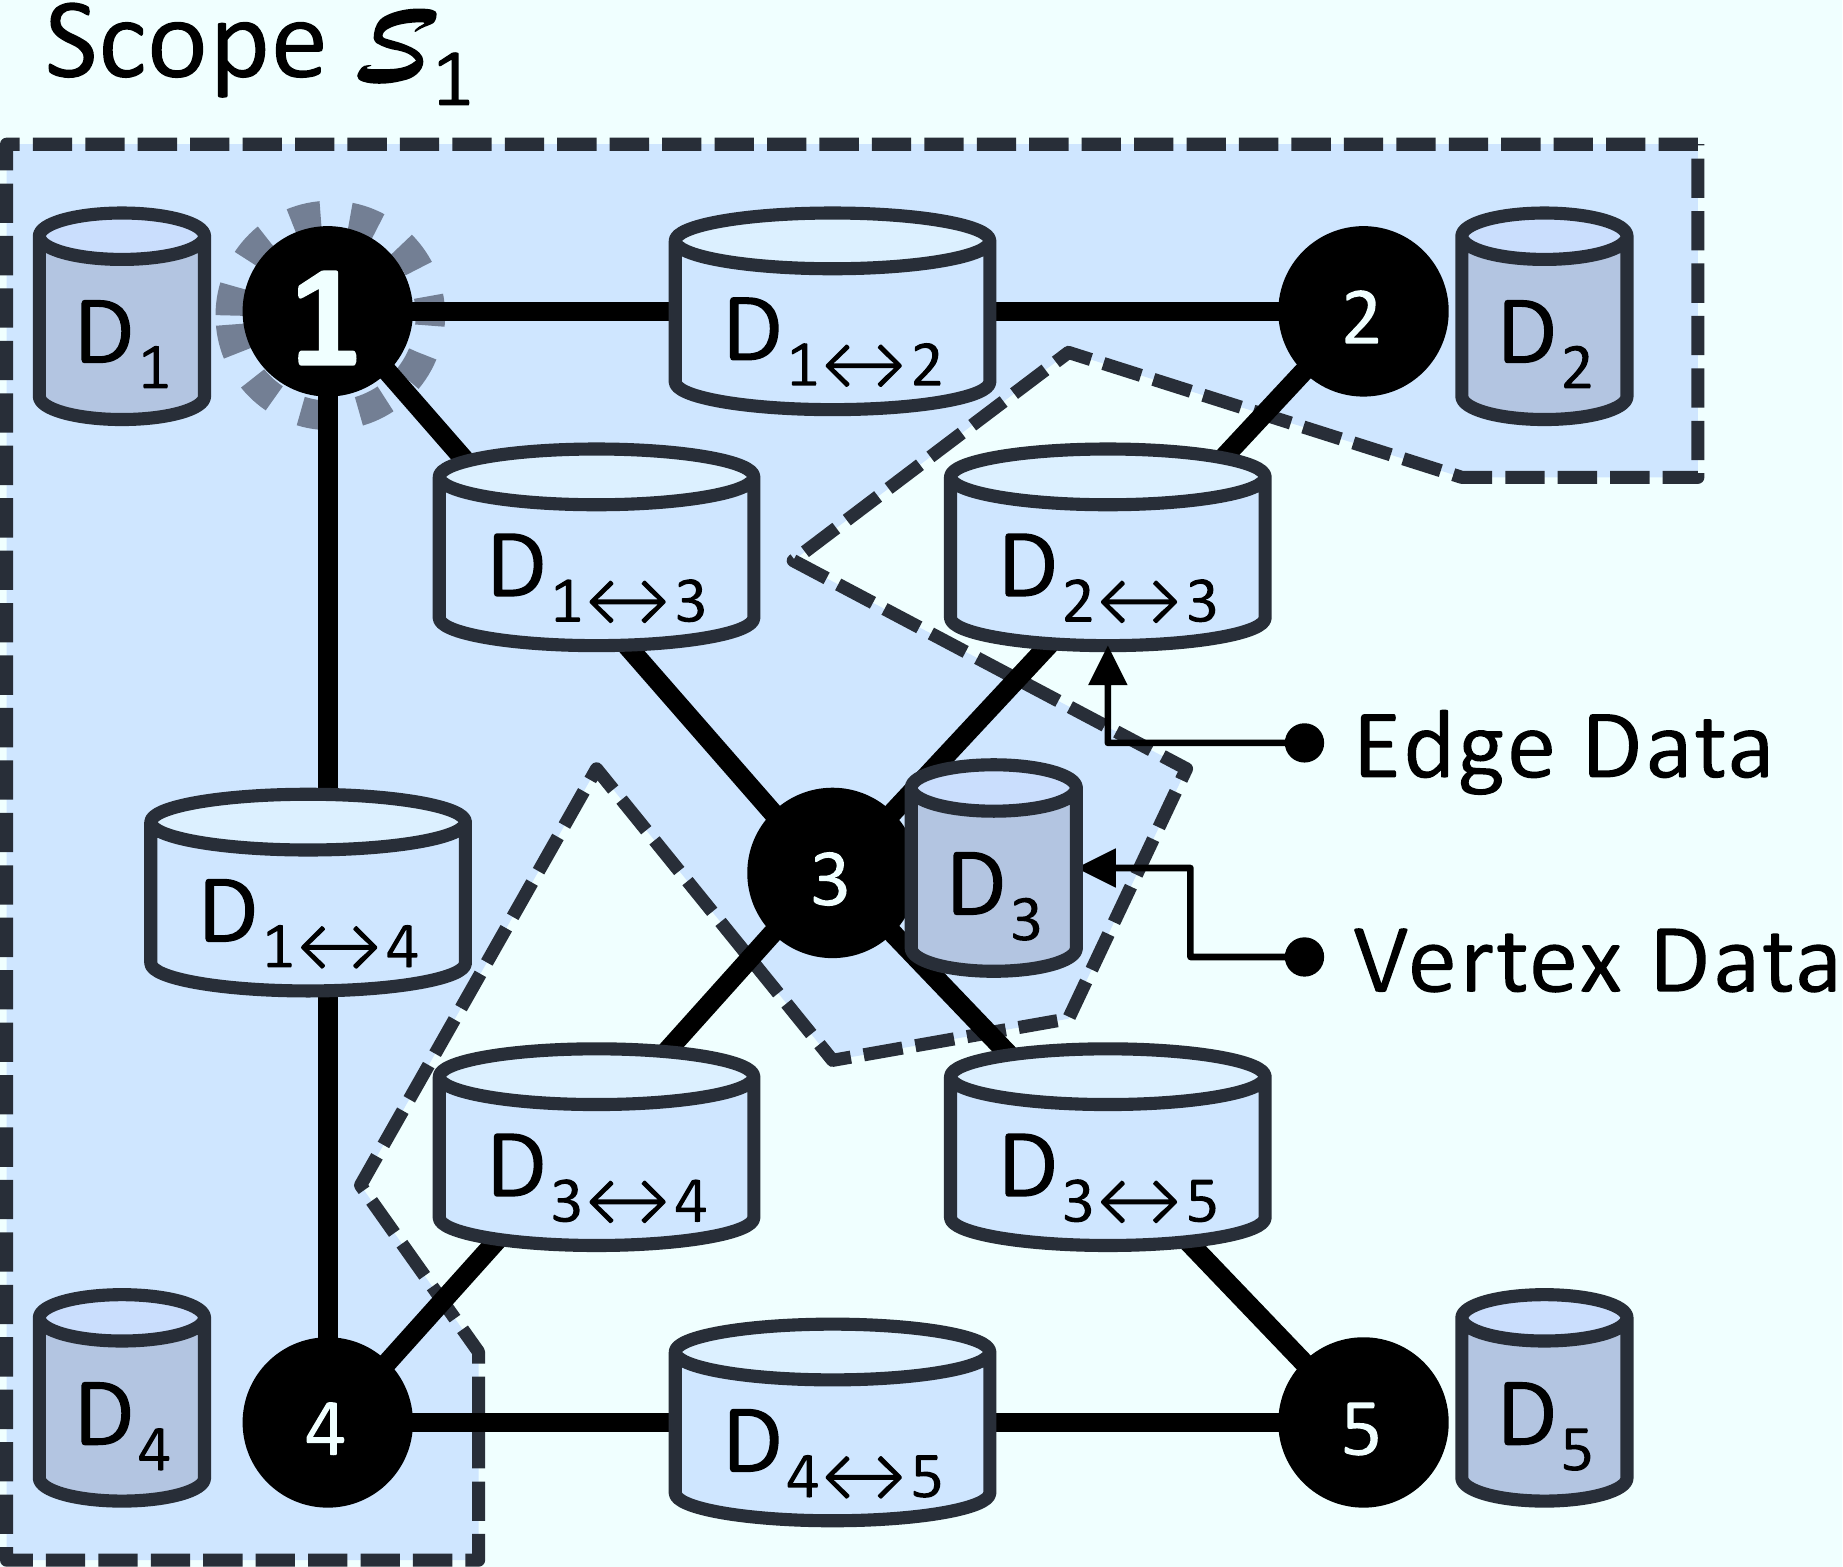
\includegraphics[width=0.7\textwidth]{../img/graphlab_model.png}
\end{center}
\end{frame}
%%%%%%%%%%%%%%%%%%%%%%%%%%%%
\begin{frame}
\frametitle{\bf The GraphLab abstraction}
\begin{center}
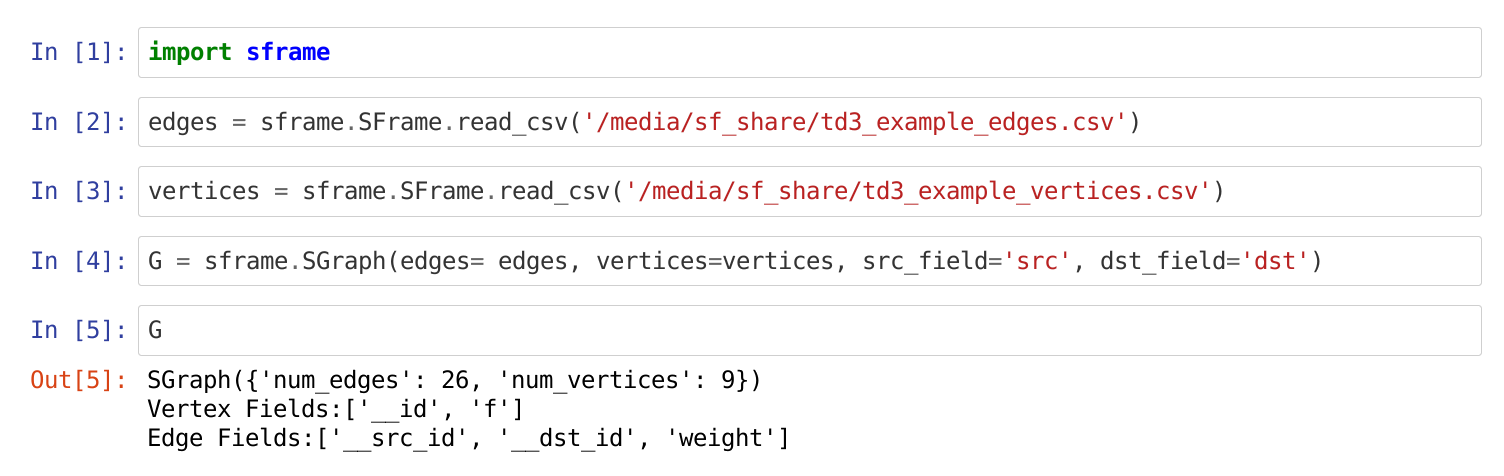
\includegraphics[width=\textwidth]{../img/load_graph.png}
\end{center}
\end{frame}
%%%%%%%%%%%%%%%%%%%%%%%%%%%%
\begin{frame}[fragile=singleslide]
\frametitle{\bf The GraphLab abstraction}
\begin{center}
Under the hood: tabular representation
\\*
\begin{tabular}{cc}
\begin{minipage}{0.4\textwidth}
\tiny
\begin{verbatim}
Columns:
    __id	int
    f	float

Rows: 9

Data:
+------+------+
| __id |  f   |
+------+------+
|  5   | 0.51 |
|  7   | 0.82 |
|  10  | 0.08 |
|  2   | 0.82 |
|  6   | 0.85 |
|  9   | 0.83 |
|  3   | 0.18 |
|  1   | 0.35 |
|  4   | 0.36 |
+------+------+
[9 rows x 2 columns]
\end{verbatim}
\end{minipage}
&
\begin{minipage}{0.4\textwidth}
\tiny
\begin{verbatim}
Columns:
    __src_id	int
    __dst_id	int
    weight	float

Rows: 26

Data:
+----------+----------+----------+
| __src_id | __dst_id |  weight  |
+----------+----------+----------+
|    7     |    5     | 0.13185  |
|    5     |    7     | 0.13185  |
|    7     |    7     | 0.026779 |
|    10    |    7     | 0.57121  |
|    7     |    10    | 0.57121  |
|    10    |    2     | 0.94047  |
|    7     |    6     | 0.64528  |
|    5     |    3     | 0.93374  |
|    10    |    3     | 0.31713  |
|    5     |    1     | 0.57796  |
+----------+----------+----------+
[26 rows x 3 columns]
Note: Only the head of the SFrame is printed.
\end{verbatim}
\end{minipage}
\end{tabular}

\end{center}
\end{frame}
%%%%%%%%%%%%%%%%%%%%%%%%%%%%
\begin{frame}[t]
\frametitle{\bf The GraphLab abstraction}
\begin{center}
\only<1>{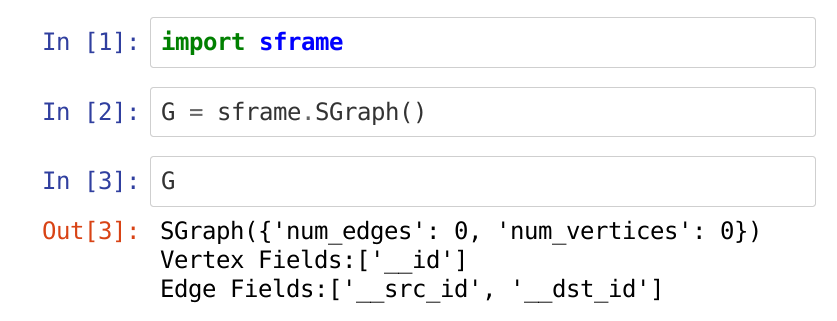
\includegraphics[width=0.75\textwidth]{../img/immutable_1.png}\vfill}
\only<2>{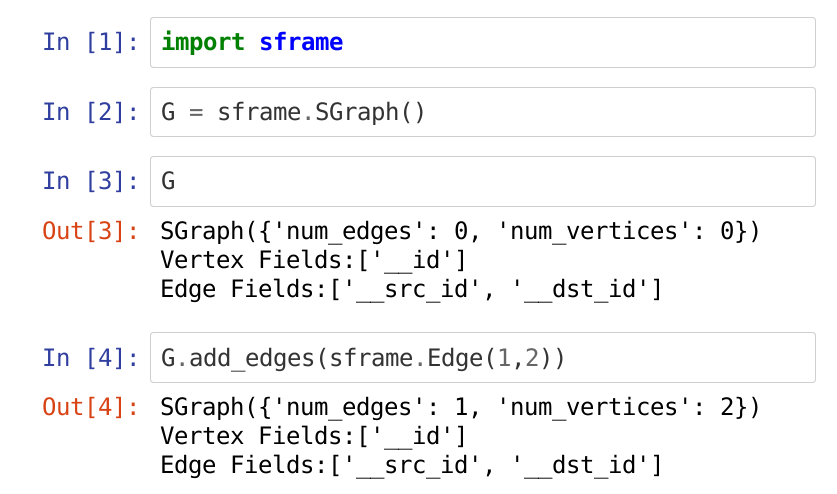
\includegraphics[width=0.75\textwidth]{../img/immutable_2.png}\vfill}
\only<3>{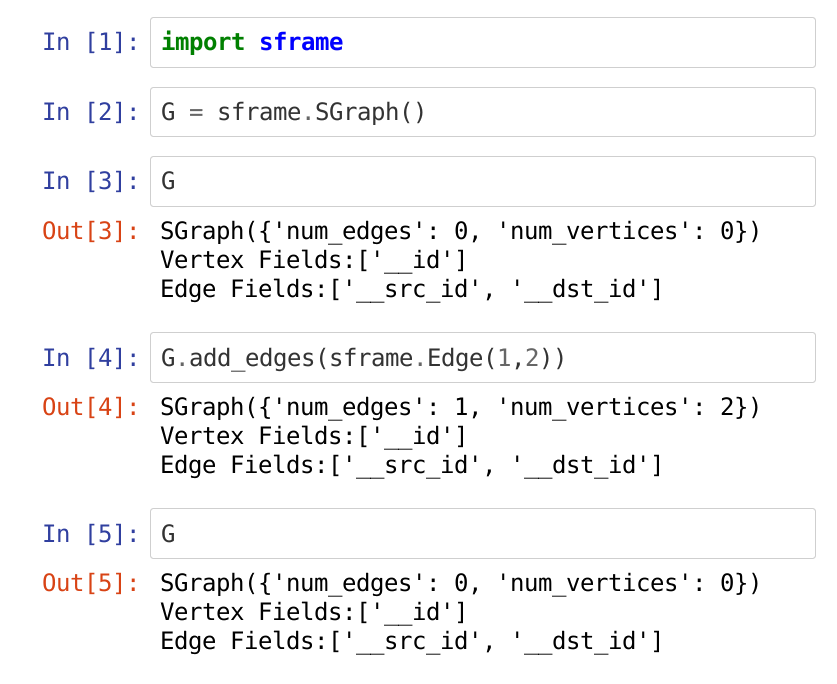
\includegraphics[width=0.75\textwidth]{../img/immutable_3.png}\vfill}
\end{center}
\end{frame}
%%%%%%%%%%%%%%%%%%%%%%%%%%%%
\begin{frame}
\frametitle{\bf The GraphLab abstraction}
\begin{center}
\begin{itemize}[<+-| alert@+>]
    \item The graph is immutable. \questionbox{why?}
    \item \yellbox{All computations are executed asyncronously}
    \consindent{We do not know the order of execution
    \item[] We do not even know where the node is stored \questionbox{what data can we access?}}
    \item The data is stored in the graph itself
    \consindent{only access \yellbox{local data}}
    \item Functional programming approach
\end{itemize}
\end{center}
\end{frame}
%%%%%%%%%%%%%%%%%%%%%%%%%%%%

\begin{frame}[fragile]
\frametitle{\bf The GraphLab abstraction}
\begin{lstlisting}[basicstyle=\fdmfamily\scriptsize, stepnumber = 0]
triple_apply(triple_apply_fn, mutated_fields, input_fields=None)
\end{lstlisting}

\vspace{-1.5\baselineskip}
processes all edges asyncronously and in parallel
\begin{lstlisting}[basicstyle=\fdmfamily\scriptsize, stepnumber = 0]
>>> PARALLEL FOR (source, edge, target) AS triple in G:
\dots     LOCK (triple.source, triple.target)
\dots     (source, edge, target) = triple_apply_fn(triple)
\dots     UNLOCK (triple.source, triple.target)
\dots END PARALLEL FOR
\end{lstlisting}

\vspace{-1.5\baselineskip}
\begin{itemize}[<+->]
\item \questionbox{No guarantees on order of execution}
\item \questionbox{Updating {\footnotesize \path{(src, edge, dst)}} violates immutability}
\item {\footnotesize \path{triple_apply_fn}} receives a copy of {\footnotesize \path{(src, edge, dst)}}
\consindent{ returns an updated {\footnotesize \path{(src', edge', dst')}}
\item[] use return values to \yellbox{build a new graph}
}
\end{itemize}
\end{frame}

%%%%%%%%%%%%%%%%%%%%%%%%%%%%
\begin{frame}[fragile]
\frametitle{\bf The GraphLab abstraction}
\begin{center}
\yellbox{{\footnotesize \path{triple_apply_fn}} is a pure function}
\end{center}

Function in the mathematical sense, same input gives same output.

\begin{lstlisting}[basicstyle=\fdmfamily\scriptsize]
def triple_apply_fn(src, edge, dst):
    #can only access data stored in src, edge, and dst,
    #three dictionaries containing a copy of the
    #fields indicated in mutated_fields
    f = dst['f']

    #inputs are copies, this does not change original edge
    edge['weight'] = g(f)

    return ({'f': dst['f']}, edge, dst)
\end{lstlisting}

\end{frame}
%%%%%%%%%%%%%%%%%%%%%%%%%%%%
\begin{frame}[fragile]
\frametitle{\bf The GraphLab abstraction}
\begin{center}
An example, computing degree of nodes
\end{center}

\begin{lstlisting}[basicstyle=\fdmfamily\scriptsize]
def degree_count_fn (src, edge, dst):
    src['degree'] += 1
    dst['degree'] += 1
    return (src, edge, dst)

G_count = G.triple_apply(degree_count_fn, 'degree')
\end{lstlisting}
\end{frame}

\begin{frame}[t, fragile]
\frametitle{\bf The GraphLab abstraction}
\begin{center}
\vspace{-1\baselineskip}
Slightly more complicated example, suboptimal pagerank
\vspace{-0.5\baselineskip}
\end{center}
\begin{lstlisting}[basicstyle=\fdmfamily\scriptsize]
#assume each node in G has a field 'degree' and 'pagerank'
#initialize 'pagerank' = 1/n for all nodes

def weight_count_fn (src, edge, dst):
    dst['degree'] += edge['weight']
    return (src, edge, dst)

def pagerank_step_fn (src, edge, dst):
    dst['pagerank'] += (edge['weight']*src['pagerank']
                                      /dst['degree'])
    return (src, edge, dst)

G_pagerank = G.triple_apply(weight_count_fn, 'degree')

while not converged(G_pagerank):
    G_pagerank = G_pagerank.triple_apply(
                        pagerank_step_fn, 'pagerank')
\end{lstlisting}
\pause

\begin{center}
\vspace{-1.5\baselineskip}
\questionbox{How many iterations to convergence?}
\end{center}
\end{frame}

%%%%%%%%%%%%%%%%%%%%%%%%%%%

\begin{frame}[allowframebreaks]
\frametitle{Bibliography}
\nocite{low2010graphlab:}
\printbibliography
\end{frame}


%%%%%%%%%%%%%%%%%%%%%%%%%%%%


\MakeLastSlide
\end{document}
